\documentclass[a4paper]{article}
\usepackage[a4paper,margin=0mm]{geometry}
\usepackage{fontspec}
\usepackage{unicode-math}
\usepackage{tikz}
\usepackage[table]{xcolor}
\usepackage[absolute]{textpos}
\usepackage{enumitem}
\usepackage{array}
\usepackage{multirow}

\setmainfont{Libertinus Serif}
\setsansfont{Libertinus Sans}
\setmathfont{Libertinus Math}
\newfontfamily\trackedsans{Libertinus Sans}[LetterSpace=8.0]

\definecolor{accent}{HTML}{602785}
\definecolor{badge}{HTML}{B8A0C8}
\definecolor{ink}{HTML}{2A2E30}

\setlength{\TPHorizModule}{1mm}
\setlength{\TPVertModule}{1mm}
\setlength{\parindent}{0pt}
\pagestyle{empty}

% ---- Safe print margins: 16mm outer on both sides so bound/trimmed copies never
% clip problem text. Columns are 83mm wide with a 6mm gap on each side of the
% center rule (at x=105mm). ----
\newcommand{\LCOL}{16mm}
\newcommand{\RCOL}{111mm}
\newcommand{\COLW}{83mm}

% ---- Plain topic header: number chip + title, thin rule underneath. No band, no watermark. ----
\newcommand{\topicheader}[2]{%
\begin{textblock*}{194mm}(16mm,10mm)
\begin{tikzpicture}
\node[fill=accent,text=white,font=\sffamily\bfseries\fontsize{13}{13}\selectfont,
      minimum width=9mm,minimum height=9mm,inner sep=0pt] at (4.5mm,-4.5mm) {#1};
\node[font=\sffamily\bfseries\fontsize{15}{16}\selectfont,text=ink,anchor=west] at (12mm,-4.5mm) {#2};
\end{tikzpicture}
\end{textblock*}
\begin{textblock*}{194mm}(16mm,22.5mm)

\begin{tikzpicture}
\fill[accent] (0,0) rectangle (194mm,0.5mm);
\end{tikzpicture}
\end{textblock*}
}

\newcommand{\pagefooter}[1]{%
\begin{textblock*}{194mm}(8mm,286.41mm)
  
\begin{tikzpicture}
    \fill[accent] (0,0) rectangle (194mm,0.6mm);
  \end{tikzpicture}
\end{textblock*}
\begin{textblock*}{63.59mm}(8mm,288.27mm)
  {\sffamily\bfseries\color{accent}\fontsize{13}{16}\selectfont SAT 1200+}
\end{textblock*}
\begin{textblock*}{10mm}(188mm,288.27mm)
  \centering{\sffamily\color{accent}\fontsize{14}{16}\selectfont #1}
\end{textblock*}
}

% ---- Fixed-length vertical column rule: #1 = top y (mm), #2 = length (mm) ----
\newcommand{\colrule}[2]{%
\begin{textblock*}{1mm}(105mm,#1mm)
\begin{tikzpicture}
\draw[black!65,line width=0.5pt] (0,0) -- (0,#2mm);
\end{tikzpicture}
\end{textblock*}
}

\newcommand{\setkicker}[2]{%
{\sffamily\bfseries\fontsize{12}{14}\selectfont #1.}\ {\itshape\fontsize{11}{14}\selectfont\color{black!75} #2}\par\vspace{2mm}%
}

% ---- Small boxed problem number, reference-style. Plain \fbox -- stays flush with
% the text baseline instead of centering on it. ----
\setlength{\fboxsep}{1.4pt}
\setlength{\fboxrule}{0.5pt}
\newcommand{\pnum}[1]{\fcolorbox{ink}{white}{\sffamily\bfseries\fontsize{8}{8}\selectfont #1}~}

% ---- QR placeholder square + caption below ----
\newcommand{\qrbox}[1]{%
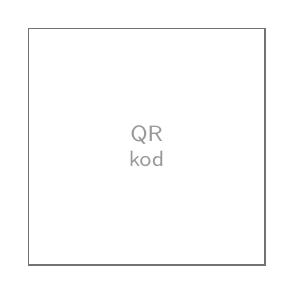
\begin{tikzpicture}
\draw[black!55,line width=0.6pt] (0,0) rectangle (30mm,30mm);
\node[black!40,font=\sffamily\fontsize{8}{9}\selectfont,align=center] at (15mm,15mm) {QR\\kod};
\end{tikzpicture}\\[1.5mm]
{\sffamily\fontsize{9}{11}\selectfont\color{black!70} #1}%
}

% ---- Answer-table styling: accent-colored grid, like the reference "Number | Answer" table ----
\arrayrulecolor{accent}
\setlength{\arrayrulewidth}{0.7pt}
\renewcommand{\arraystretch}{1.35}
\newcommand{\anstitle}[1]{{\sffamily\bfseries\color{accent}\fontsize{11}{13}\selectfont #1}\\[1.3mm]}

\begin{document}

% ================= PAGE 1: Set 1 | Set 2 =================
\topicheader{2}{Chiziqli tenglamalar sistemasi}
\pagefooter{1}
\colrule{32}{238}
\mbox{}%

\begin{textblock*}{\COLW}(\LCOL,32mm)
{\fontsize{11.5}{14}\selectfont
\setkicker{1-to'plam}{O'rniga qo'yish usuli bilan $(x,y)$ ni toping.}

\noindent\pnum{1} $y=x+3,\quad 2x+y=18$\\[28mm]
\noindent\pnum{2} $y=2x,\quad x+y=15$\\[28mm]
\noindent\pnum{3} $y=3x-4,\quad x+y=12$\\[28mm]
\noindent\pnum{4} $x=y+5,\quad 2y+x=17$\\[28mm]
\noindent\pnum{5} $y=-x+10,\quad 3x-y=2$\\[28mm]
\noindent\pnum{6} $y=4x-3,\quad 2x+y=21$
}
\end{textblock*}

\begin{textblock*}{\COLW}(\RCOL,32mm)
{\fontsize{11.5}{14}\selectfont
\setkicker{2-to'plam}{Qo'shish (eliminatsiya) usuli -- ba'zilarida avval ko'paytirish kerak.}

\noindent\pnum{1} $x+y=9,\quad x-y=3$\\[28mm]
\noindent\pnum{2} $2x+y=13,\quad x-y=2$\\[28mm]
\noindent\pnum{3} $3x+2y=17,\quad x-2y=-5$\\[28mm]
\noindent\pnum{4} $2x+3y=13,\quad 4x-y=5$\\[28mm]
\noindent\pnum{5} $5x+2y=19,\quad 3x-2y=5$\\[28mm]
\noindent\pnum{6} $x+3y=14,\quad 2x+y=13$
}
\end{textblock*}

\clearpage

% ================= PAGE 2: Set 3 | Set 4 =================
\topicheader{2}{Chiziqli tenglamalar sistemasi}
\pagefooter{2}
\colrule{32}{238}
\mbox{}%

\begin{textblock*}{\COLW}(\LCOL,32mm)
{\fontsize{11.5}{14}\selectfont
\setkicker{3-to'plam}{Aralash -- qaysi usul qulayroq, shuni tanlang.}

\noindent\pnum{1} $y=3x-5,\quad 2x+3y=18$\\[28mm]
\noindent\pnum{2} $4x-y=10,\quad 2x+y=14$\\[28mm]
\noindent\pnum{3} $x+y=20,\quad x-y=-6$\\[28mm]
\noindent\pnum{4} $3x+y=7,\quad y=x-5$\\[28mm]
\noindent\pnum{5} $2x+5y=22,\quad x-y=4$\\[28mm]
\noindent\pnum{6} $6x-2y=24,\quad 3x+y=18$
}
\end{textblock*}

\begin{textblock*}{\COLW}(\RCOL,32mm)
{\fontsize{11}{13.5}\selectfont
\setkicker{4-to'plam}{Har bir sistemani tasniflang: \textbf{bitta yechim} (uni toping), \textbf{yechimsiz}, yoki \textbf{cheksiz ko'p yechim}.}

\noindent\pnum{1} $3x+6y=12,\quad x+2y=4$\\[20mm]
\noindent\pnum{2} $x+2y=5,\quad 2x+4y=9$\\[20mm]
\noindent\pnum{3} $x-3y=1,\quad 2x-6y=2$\\[20mm]
\noindent\pnum{4} $5x+y=10,\quad x-y=2$\\[20mm]

$k$ ning qiymatini toping:

\noindent\pnum{5} $2x+ky=6$ va $4x+8y=20$ sistemasi \textbf{yechimga ega bo'lmasligi} uchun $k=$?\\[14mm]
\noindent\pnum{6} $x+3y=6$ va $2x+ky=12$ sistemasi \textbf{cheksiz ko'p yechimga ega bo'lishi} uchun $k=$?
}
\end{textblock*}

\clearpage

% ================= PAGE 3: Set 5 | Set 6 (spot the error) =================
\topicheader{2}{Chiziqli tenglamalar sistemasi}
\pagefooter{3}
\colrule{32}{238}
\mbox{}%

\begin{textblock*}{\COLW}(\LCOL,32mm)
{\fontsize{11}{13.5}\selectfont
\setkicker{5-to'plam}{Sistemani yeching, so'ng aynan so'ralgan kattalikni toping -- shunchaki $x$ yoki $y$ emas.}

\noindent\pnum{1} $x+y=14,\ x-y=4$ -- $xy$ ni toping.\\[34mm]
\noindent\pnum{2} $2x+y=11,\ x-y=1$ -- $x+y$ ni toping.\\[34mm]
\noindent\pnum{3} $x+2y=16,\ x-y=1$ -- $2x-y$ ni toping.\\[34mm]
\noindent\pnum{4} $3x+y=19,\ x+y=9$ -- $x-y$ ni toping.\\[34mm]
\noindent\pnum{5} $x+y=13,\ 2x-y=8$ -- $x^2-y^2$ ni toping.
}
\end{textblock*}

\begin{textblock*}{\COLW}(\RCOL,32mm)
{\fontsize{10.5}{13.5}\selectfont
\setkicker{6-to'plam}{Xatoni toping -- buzilgan qadamni ayting, to'g'ri javobni bering.}

\noindent\pnum{1} $x+y=8,\ x-y=2$ ifodasida ko'rsatilgan yechimda xato bor:\\[1mm]
\hspace*{7mm}\textit{``Qo'shib: $2x=8-2=6$, demak $x=3$, $y=5$.''}\\[2mm]
\hspace*{7mm}Xato va to'g'ri javob: \makebox[52mm]{\dotfill}\\[8mm]

\noindent\pnum{2} $2x+y=7,\ y=3x-8$ ifodasida ko'rsatilgan yechimda xato bor:\\[1mm]
\hspace*{7mm}\textit{``$2x+3x-8=7$, demak $5x=7$, $x=\frac{7}{5}$.''}\\[2mm]
\hspace*{7mm}Xato va to'g'ri javob: \makebox[52mm]{\dotfill}\\[8mm]

\noindent\pnum{3} $4x+2y=8,\ 2x+y=5$ ifodasida ko'rsatilgan yechimda xato bor:\\[1mm]
\hspace*{7mm}\textit{``Ikkala tenglama ham bitta chiziqni ifodalaydi, shuning uchun cheksiz ko'p yechim bor.''}\\[2mm]
\hspace*{7mm}Xato va to'g'ri javob: \makebox[52mm]{\dotfill}\\[8mm]

\noindent\pnum{4} $3x-y=5,\ x+y=11$ ifodasida ko'rsatilgan yechimda xato bor:\\[1mm]
\hspace*{7mm}\textit{``Qo'shib: $4x=16$, $x=4$; so'ng $y=11+4=15$.''}\\[2mm]
\hspace*{7mm}Xato va to'g'ri javob: \makebox[52mm]{\dotfill}
}
\end{textblock*}

\clearpage

% ================= PAGE 4: Set 7 (bonus) -- own page; answers follow on a fresh page =================
\topicheader{2}{Chiziqli tenglamalar sistemasi}
\pagefooter{4}
\colrule{32}{238}
\mbox{}%

\begin{textblock*}{\COLW}(\LCOL,32mm)
{\fontsize{11.5}{14}\selectfont
\setkicker{7-to'plam}{Bonus / qiyin -- har biriga taxminan 90 soniya.}

\noindent\pnum{1} $2x+3y=7,\quad 5x-2y=8$\\[36mm]
\noindent\pnum{2} Ikki sonning yig'indisi $24$, ayirmasi $8$ ga teng. Bu ikki son nechaga teng?\\[36mm]
\noindent\pnum{3} $3x+ky=10$ va $x+2y=3$ sistemasi \textbf{yechimga ega bo'lmasligi} uchun $k=$?\\[36mm]
\noindent\pnum{4} $4x+3y=25,\quad 2x-y=5$
}
\end{textblock*}

\clearpage

% ================= PAGE 5: Javoblar -- full-page answer tables, own page always =================
\topicheader{2}{Chiziqli tenglamalar sistemasi}
\pagefooter{5}
\mbox{}%

\begin{textblock*}{194mm}(16mm,30mm)
{\bfseries\itshape\color{accent}\fontsize{19}{21}\selectfont\centering Javoblar\par}
\end{textblock*}

\begin{textblock*}{194mm}(16mm,44mm)
{\fontsize{9.5}{12}\selectfont
\centering
\renewcommand{\arraystretch}{1.3}
\begin{tabular}{|>{\centering\arraybackslash}p{24mm}|>{\centering\arraybackslash}p{9mm}|>{\centering\arraybackslash}p{40mm}|>{\centering\arraybackslash}p{9mm}|>{\centering\arraybackslash}p{40mm}|}
\hline
\rowcolor{badge!55}\textbf{To'plam} & \textbf{\#} & \textbf{Javob} & \textbf{\#} & \textbf{Javob}\\
\hline
\multirow{3}{24mm}{\centering 1-to'plam} & 1 & $(5,8)$ & 2 & $(5,10)$\\\cline{2-5}
 & 3 & $(4,8)$ & 4 & $(9,4)$\\\cline{2-5}
 & 5 & $(3,7)$ & 6 & $(4,13)$\\\hline
\multirow{3}{24mm}{\centering 2-to'plam} & 1 & $(6,3)$ & 2 & $(5,3)$\\\cline{2-5}
 & 3 & $(3,4)$ & 4 & $(2,3)$\\\cline{2-5}
 & 5 & $(3,2)$ & 6 & $(5,3)$\\\hline
\multirow{3}{24mm}{\centering 3-to'plam} & 1 & $(3,4)$ & 2 & $(4,6)$\\\cline{2-5}
 & 3 & $(7,13)$ & 4 & $(3,-2)$\\\cline{2-5}
 & 5 & $(6,2)$ & 6 & $(5,3)$\\\hline
\multirow{6}{24mm}{\centering 4-to'plam} & \multicolumn{4}{p{98mm}|}{1.\ Cheksiz ko'p yechim (2-tenglama 1-tenglamaning aynan $\frac13$ qismi).}\\\cline{2-5}
 & \multicolumn{4}{p{98mm}|}{2.\ Yechimsiz (koeffitsient nisbati ikkala marta ham $2$, lekin $5\times2=10\ne9$).}\\\cline{2-5}
 & \multicolumn{4}{p{98mm}|}{3.\ Cheksiz ko'p yechim (2-tenglama 1-tenglamaning aynan $2$ bar\-obari).}\\\cline{2-5}
 & \multicolumn{4}{p{98mm}|}{4.\ Bitta yechim: $(x,y)=(2,0)$.}\\\cline{2-5}
 & \multicolumn{4}{p{98mm}|}{5.\ $k=4$}\\\cline{2-5}
 & \multicolumn{4}{p{98mm}|}{6.\ $k=6$}\\\hline
\multirow{5}{24mm}{\centering 5-to'plam} & \multicolumn{4}{p{98mm}|}{1.\ $xy=45$ ($x=9,y=5$)}\\\cline{2-5}
 & \multicolumn{4}{p{98mm}|}{2.\ $x+y=7$ ($x=4,y=3$)}\\\cline{2-5}
 & \multicolumn{4}{p{98mm}|}{3.\ $2x-y=7$ ($x=6,y=5$)}\\\cline{2-5}
 & \multicolumn{4}{p{98mm}|}{4.\ $x-y=1$ ($x=5,y=4$)}\\\cline{2-5}
 & \multicolumn{4}{p{98mm}|}{5.\ $x^2-y^2=13$ ($x=7,y=6$)}\\\hline
\multirow{4}{24mm}{\centering 6-to'plam} & \multicolumn{4}{p{98mm}|}{1.\ Xato -- $8+2$ o'rniga $8-2$ ishlatilgan. To'g'ri: $2x=10$, $x=5$, $y=3$.}\\\cline{2-5}
 & \multicolumn{4}{p{98mm}|}{2.\ Xato -- $-8$ had o'ng tomonga ko'chirilmagan. To'g'ri: $5x-8=7$, $x=3$, $y=1$.}\\\cline{2-5}
 & \multicolumn{4}{p{98mm}|}{3.\ Xato -- konstantalar tekshirilmagan: nisbat mos kelmaydi ($8$ vs $10$) -- demak \textbf{yechimsiz}, cheksiz ko'p emas.}\\\cline{2-5}
 & \multicolumn{4}{p{98mm}|}{4.\ Xato -- ishora: $y=11-4=7$ bo'lishi kerak edi, $(4,7)$.}\\\hline
\multirow{4}{24mm}{\centering 7-to'plam} & 1 & $(2,1)$ & \multicolumn{2}{p{49mm}|}{2.\ Sonlar: $16$ va $8$}\\\cline{2-5}
 & \multicolumn{4}{p{98mm}|}{3.\ $k=6$}\\\cline{2-5}
 & 4 & $(4,3)$ & -- & --\\\hline
\end{tabular}
}
\end{textblock*}

\begin{textblock*}{194mm}(16mm,220mm)
\centering
{\sffamily\fontsize{9.5}{11.5}\selectfont\color{black!70} Video yechimlar va qo'shimcha testlar uchun quyidagi QR kodlarni skanerlang:}\\[4mm]
\begin{minipage}[t]{32mm}\centering\qrbox{YouTube}\end{minipage}%
\hspace{16mm}%
\begin{minipage}[t]{32mm}\centering\qrbox{Telegram}\end{minipage}
\end{textblock*}

\end{document}
